
% This is a simple template for a LaTeX document using the "article" class.
% See "book", "report", "letter" for other types of document.

\documentclass[11pt]{article} % use larger type; default would be 10pt

\usepackage[T1]{fontenc}
\usepackage[french]{babel}
\usepackage[utf8]{inputenc} % set input encoding (not needed with XeLaTeX)
\usepackage{kpfonts}

%%% Examples of Article customizations
% These packages are optional, depending whether you want the features they provide.
% See the LaTeX Companion or other references for full information.

%%% PAGE DIMENSIONS
\usepackage{geometry} % to change the page dimensions
\geometry{a4paper} % or letterpaper (US) or a5paper or....
% \geometry{margin=2in} % for example, change the margins to 2 inches all round
% \geometry{landscape} % set up the page for landscape
%   read geometry.pdf for detailed page layout information


% \usepackage[parfill]{parskip} % Activate to begin paragraphs with an empty line rather than an indent

%%% PACKAGES
\usepackage{booktabs} % for much better looking tables
\usepackage{array} % for better arrays (eg matrices) in maths
\usepackage{paralist} % very flexible & customisable lists (eg. enumerate/itemize, etc.)
\usepackage{verbatim} % adds environment for commenting out blocks of text & for better verbatim
% \usepackage{subfig} % make it possible to include more than one captioned figure/table in a single float
% These packages are all incorporated in the memoir class to one degree or another...

%%% HEADERS & FOOTERS
\usepackage{fancyhdr} % This should be set AFTER setting up the page geometry
\pagestyle{fancy} % options: empty , plain , fancy

\usepackage{graphicx} % support the \includegraphics command and options
\usepackage{subcaption}
\usepackage{caption}

\fancyhf{}
% \rhead{La Compilation}
\lhead{Optimisation du GCC}
% \rfoot{Page \thepage}
\cfoot{\thepage}

% \renewcommand{\headrulewidth}{0pt} % customise the layout...
% \lhead{}\chead{}\rhead{}
% \lfoot{}\cfoot{\thepage}\rfoot{}

%%% SECTION TITLE APPEARANCE
\usepackage{sectsty}
\allsectionsfont{\sffamily\mdseries\upshape} % (See the fntguide.pdf for font help)
% (This matches ConTeXt defaults)

%%% ToC (table of contents) APPEARANCE
\usepackage[nottoc,notlof,notlot]{tocbibind} % Put the bibliography in the ToC
\usepackage[titles,subfigure]{tocloft} % Alter the style of the Table of Contents
\renewcommand{\cftsecfont}{\rmfamily\mdseries\upshape}
\renewcommand{\cftsecpagefont}{\rmfamily\mdseries\upshape} % No bold!

%%% END Article customizations

%%% The "real" document content comes below...

\title{Optimisation du code par GCC}
\author{Evan VOYLES, Amaury RODRIGUEZ, Stefan GA\L KIEWICZ}
%\date{} % Activate to display a given date or no date (if empty),
         % otherwise the current date is printed

\begin{document}
\maketitle

\section*{Notions de compilation}
Il y a une puissance particuli\`ere caché derrière les trois lettres \verb|gcc| - signifiant à la fois
la `Gnu Compiler Collection' et la commande à lancer dans le terminal pour compiler un program C. Enfin pas que.
Quand on appelle une commande de la forme
% { \centering
\begin{verbatim}

    gcc -o hello hello_world.c
\end{verbatim}
on lance effectivement une multitude de processus qui travaillent scrupuleusement en silence.
Il s'agit de:
\begin{enumerate}
    \item Préprocesser le fichier .c
    \item Compiler les fichiers processés pour créer des fichier d'objet (.o)
    \item Relier des fichiers d'objet dans une éxécutable
\end{enumerate}

Ca veut dire quoi, préprocesser un fichier .c ? En effet, à chaque fois qu'on
écrit \verb|#include <stdio.h>| pour inclure un fichier d'entête, avant la compilation
un outil dit le préprocesseur va remplacer une ligne d'include avec tout le contenu du fichier d'entête.
Alors la directive préprocesseur \verb|#include| consiste en une opération de copier et coller. Il y a plusieurs autres directives qui sont processées avant de compiler,
par exemple le lecteur reconnaitra peut-etre les directives
\begin{verbatim}
    #if, #ifdef, #ifndef, #else, #elif
\end{verbatim}
qui sont employées
pour la compilation conditionnelle (par exemple, inclure un fichier spécifique pour Windows si le système est Windows)
où bien pour éviter d'inclure le même fichier plusiers fois:
\begin{verbatim}
    #ifndef MONFICHIER_H
    #define MONFICHIER_H

    / Contenu du fichier monfichier.h /

    ...

    #endif
\end{verbatim}

Après que nos fichiers sont préprocessés, ils sont prêts pour être compilés. La compilation traduit des fichiers en C à des instructions de machine
en binaire, dit des fichiers d'objet qui portent l'extension .o. Pour experimenter chez vous, on peut donner l'option \verb|-c| à gcc pour arrêter après
le compilation et créer des fichiers d'objet.
    Lors de la derniere étape, il s'agit de regrouper tout les fichiers d'objet pertinents et de les emballer dans un seul exécutable. C'est quoi la différence concrète entre
un `programme' C et une `bibliothèque' ? Une bibliothèque c'est une collection des fonctions et leur définitions tandis ce que un programme contient la fonction spécial
\verb|main|, qui sert comme une porte d'entrée de l'exécution d'un programme.

    Alors finalement l'outil \verb|ld|, dit le `linker' en anglais, relie tous les fichiers .o dans un executable. Son travail est compliqué mais fondamental. Grosso modo, \verb|ld|
trouve exactement où sont définies les fonctions extérieures qu'on appelle dans un programme. Par exemple, pour un programme simple HelloWorld on va utiliser la fonction \verb|printf| qui
est définie d'ailleurs. Au moment de créer l'exécutable, \verb|ld| va chercher la définition de \verb|printf| dans la bibliothèque standard et mettre les instructions binaires dans l'exécutable.
La magie de \verb|gcc| c'est qu'il a fait tout cela pour vous en coulisse - un vrai emploi ingrat.
% \fancyhf{}
% \rhead{La Compilation}
\section*{L'Optimisation}
Pendant l'étape de compilation, le compileur peut analyser votre code et effectuer des optimisations, si vous le souhaitez.
Il y a une centaine des options pour le compileur dont au moins cinquante pour l'optimisation. Les options pour changer le comportement
d'optimisation commence par un -f, suivi par le nom de l'option. Comme il y des nombreuses optimisations spéficiques, gcc a regroupé les
stratégies d'optimisation qui ont le même objectif de compilation. C'est-à-dire que certaines optimisations pourraient rendre le code plus rapide mais
également augmenter la taille de l'exécutable. Alors les classes se divisent en différents niveaux de -O.
\subsection*{-O0}
Désactiver la plupart des optimisations.

\subsection*{-O1}
Le principe c'est de réduire le temps d'exécution aussi la taille du binaire. Au niveau -O1 la compilation est un peu plus longue mais pas beaucoup
comme a ce niveau les optimisations restent quand même simples.

Le premier niveau d'optimisation actives les options suivantes
\newpage
\begin{figure}[h!]
    \centering
    \begin{subfigure}[h!]{0.49\textwidth}
        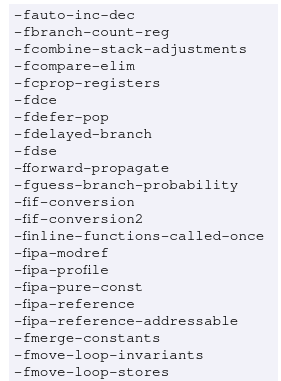
\includegraphics[height=\linewidth]{./media/O1top}
    \end{subfigure}
    \begin{subfigure}[h!]{0.49\textwidth}
        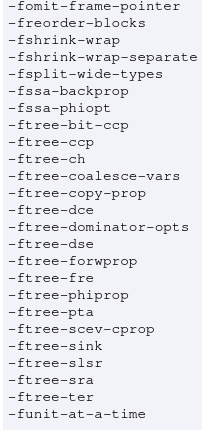
\includegraphics[height=\linewidth]{./media/O1bot}
    \end{subfigure}
\end{figure}

\subsection*{-O2}

Le deuxième niveau active plus d'optimisations. Sans échanger la taille de l'exécutable
pour la vitesse du programme, ce niveau ralentit le temps de compilation mais augmente la performance
des instructions genérées. Les options activées à ce niveau là, ce sont toutes les options de -O2 plus:

\begin{figure}[h!]
    \centering
    \begin{subfigure}[h!]{0.49\textwidth}
        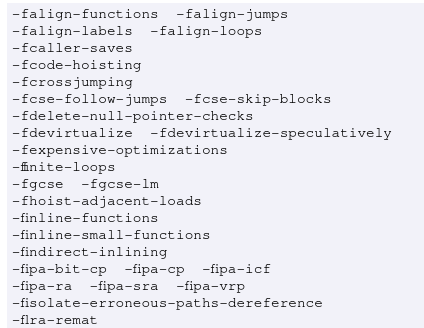
\includegraphics[height=.8\linewidth]{./media/O2top}
    \end{subfigure}
    \begin{subfigure}[h!]{0.49\textwidth}
        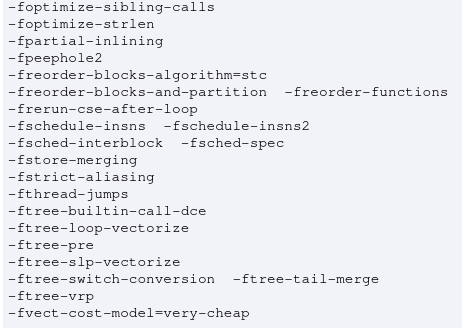
\includegraphics[height=.8\linewidth]{./media/O2bot}
    \end{subfigure}
\end{figure}

\subsection*{-O3}

Un troisième niveau active les optimisations les plus violentes et n'hésitantes pas à créer un exécutable plus grand au nom de la vitesse.
Les options activé dans ce niveau sont:
\newpage

\begin{figure}[h!]
    \centering
    \begin{subfigure}[h!]{0.49\textwidth}
        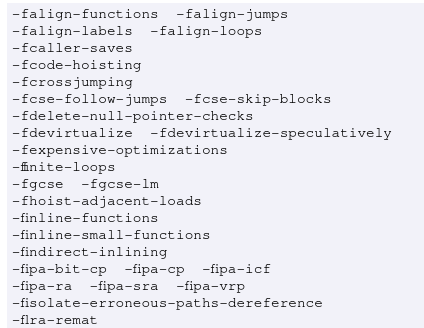
\includegraphics[height=.8\linewidth]{./media/O2top}
    \end{subfigure}
    \begin{subfigure}[h!]{0.49\textwidth}
        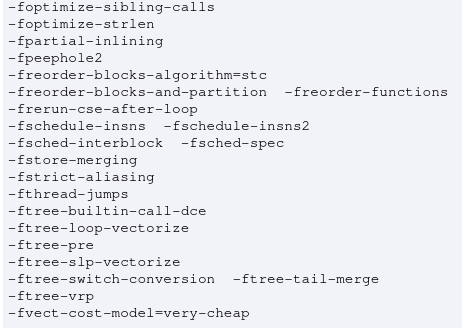
\includegraphics[height=.8\linewidth]{./media/O2bot}
    \end{subfigure}
\end{figure}


\section*{Options Sp\'ecifiques}
Comme on a vu dans le dernier section, il y a de nombreuses options activ\'e avec chaque niveau optimisation et il ne serait pas int\'eressant
de vous d\'enombrer ce que fait chacun. Donc, on va choisir juste quelques unes \`a \'etudier qui sont utilis\'e souvent.

\subsection*{Enlever le code superflu}
Pour optimiser le code le compilateur peut enlever du code redondant, en effet le but de l’optimisation du code est de réduire la taille et augmenter la vitesse d’exécution du code.
Une des premières optimisations qui paraît évidente est d’enlever le code qui ne sert pas. Il s'agit principalement de deux types du code redondant - dead code (DC, code mort) et dead storage (DS, stockage mort).
Tout segment du code qui ne s'execute pas est dit mort.

% \rhead{Code Mort}

\subsubsection*{-fdce, -ftree-dce}

\'Etudions le segment du code suivant:
\begin{verbatim}
    if (1 < 2) {
        printf("1 est plus petit que 2");
    } else {
        printf("Ca marche plus les maths");
    }
\end{verbatim}

Ici le compilateur va remarquer qu'il y a un segment de code mort et en d\'eduire que l'on peut optimiser.
Comme nous le voyons dans le code ci-dessus, la condition \verb|1 < 2| est toujours v\'erifi\'e donc la condition du \verb|if| n’a pas
besoin d’être testé et le \verb|else| ne sera jamais exécuté. Vu que la ramification d'un programme peut notoirement effectuer des
ralentissements d'\'execution, \verb|gcc| peut enlever la branche \verb|if| et effacer le code mort, sous condition que les options \verb|-fdce| et
\verb|-ftree-dce| soient activ\'ees.

En fait, l'optimisation du code mort est si importante que ca que \verb|gcc| l'enl\`eve automatiquement dans certains cas:
% \begin{figure}
    % \centering
    % \begin{subfigure}[h!]{0.4\textwidth}

\begin{figure}[h!]
    \centering
    \begin{subfigure}[h!]{0.4\textwidth}
        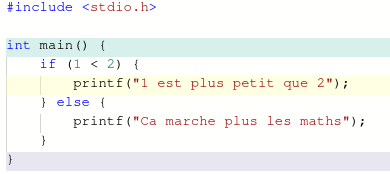
\includegraphics[width=\linewidth]{media/dce_left.png}
        % \subcaption{Code C}
    \end{subfigure}
    \begin{subfigure}[h!]{0.4\textwidth}
        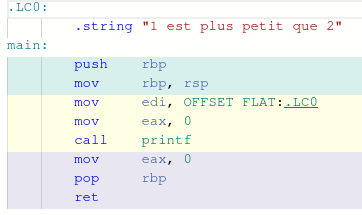
\includegraphics[width=\linewidth]{media/dce-right.png}
        % \subcaption{Assembl\'ee donn\'e par gcc}
    \end{subfigure}
    \caption{Instructions en assembl\'ee gen\'er\'ees pour x86-64 par gcc pour un program simple. Le code mort après else ne se traduit même pas.}
\end{figure}
N'ayez pas peur de l'assembl\'ee! Comme nous le pouvons constater, les instructions pour la deuxi\`eme branche de l'expression \verb|if| ne sont m\^eme
pas gen\'er\'ees (indiqu\'e par le manque de couleur surlignante la deuxième \verb|printf|)!

On peut comparer cet exemple avec un program simple similaire, mais qui diff\`ere cette fois-ci parce que le compileur ne peut pas d\'eterminer si la condition
est toujours v\'erifi\'e. \'Etudions le program suivant.


\begin{figure}[h!]
    \centering
    \begin{subfigure}[h!]{0.4\textwidth}
        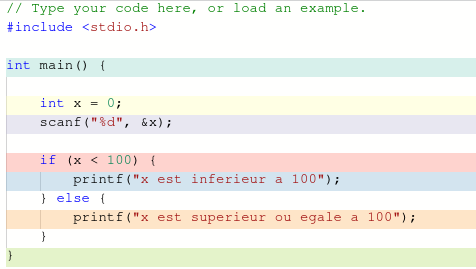
\includegraphics[width=\linewidth]{media/nodfce-left.png}
        % \subcaption{Code C}
    \end{subfigure}
    \begin{subfigure}[h!]{0.4\textwidth}
        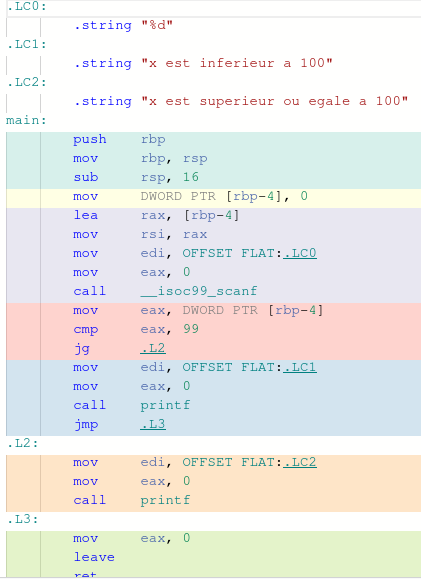
\includegraphics[width=\linewidth]{media/nodce-right.png}
        % \subcaption{Assembl\'ee donn\'e par gcc}
    \end{subfigure}
    \caption{Exemple o\`u des instructions sont gen\'er\'ees pour les deux branches du if}
\end{figure}

Vu que la condition dans le \verb|if| est dependant sur une donn\'ee d'entr\'ee qui se proc\'esse a l'ex\'ecution, il est impossible de d\'eterminer
au moment de compilation si le code est mort. Du coup, il n'y a aucun optimisation dans cet example.

\subsubsection*{-fdse, -ftree-dse}

Ces options traiten le cas o\`u il y a des variables mortes - c'est-\`a-dire des variables qui ne sont jamais acced\'ees.
Par exemple dans le code qui suit, la variable y n’est pas utilisée. Pour optimiser le code il suffit juste de retirer la ligne et ainsi
réduire la taille et augmenter la vitesse d’exécution du code. Cela marche aussi avec des fonctions qui ne font rien ou ne sont pas utilisés.

\begin{verbatim}

int my_func() {
    int x = 5;
    int y = 5;
    return x;
}
\end{verbatim}


On peut \'etudier l'assembl\'e pour visualiser les optimisation fait par gcc.

\begin{figure}[h!]
    \centering
    % \begin{subfigure}[h!]{0.3\textwidth}
    %     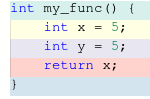
\includegraphics[width=\linewidth]{media/my_func.png}
    %     % \subcaption{Code C}
    % \end{subfigure}
    \begin{subfigure}[h!]{0.4\textwidth}
        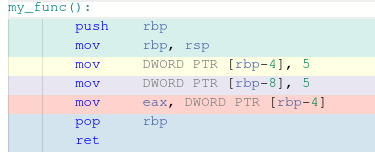
\includegraphics[width=\linewidth]{media/myfuncO0.png}
        \subcaption{-O0}
    \end{subfigure}
    \begin{subfigure}[h!]{0.4\textwidth}
        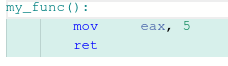
\includegraphics[width=\linewidth]{media/myfuncO1.png}
        \subcaption{-O1}
    \end{subfigure}
    \caption{Exemple o\`u le DSE est enl\`ev\'e}
\end{figure}

La fonction enti\`ere est remplac\'ee par une instruction de charger la valeur 5 dans un registre du CPU.


\section*{Optimisation des boucles}

Nous allons etudier ici quelques options qui permettent d’optimiser la compilation des boucles.


\subsection*{-fpeel-loops}
Le peeling de boucle est un cas particulier du découpage de boucle. Le découpage de boucle est une méthode d’optimisation du compilateur.
Celui-ci elimine les dépendances. Il simplifie la boucle en plusieurs boucles afin d’éliminer des dépendances. Ainsi ces boucles auront le
meme corps mais vont itérer différentes parties de la boucle. La particularité du peeling de boucle va être que si le compilateur détecte
une ou quelques itérations problématiques il va la sortir de la boucle et l’exécuter en dehors de la boucle (c’est pour cela que ca s’appelle
l’épluchage). Ainsi si l’on a par exemple 
\begin{verbatim}
int p = 10;
for (int i=0; i<10; ++i) {
    y[i] = x[i] + x[p];
    p = i;
}
\end{verbatim}
le compilateur avec fpeel-loops va remarquer que p=10 seulement a la première itération et donc il va compiler comme si le code était écris
\begin{verbatim}
y[0] = x[0] + x[10];
for (int i=1; i<10; ++i) {
   y[i] = x[i] + x[i-1];
}
\end{verbatim}
et donc on peut remarquer que le p ici n’est plus utilisé et est remplacé par directement 10 et la première
itération est sorti du corps de la boucle et est remplacé par y[0] = x[0] + x[10];

\subsection*{-fmove-loop-invariants}
Le loop invariant loop est une optimisation du compilateur qui permet de sortir un invariant d’une boucle sans changer sa semantique. Par exemple :

\begin{verbatim}
int i = 0;
while (i < n) {
    x = y + z;
    a[i] = 6 * i + x * x;
    ++i;
}
\end{verbatim}
On peut voir que x=y+z est un invariant dans la boucle et donc le fmove-loop-invariants va le sortir
 de la boucle sans en changer le sens.

\subsection*{-funswitch-loops}
le funswitch-loops est une methode d’optimisation du compilateur qui va permettre de sortir une condition situe a
linterieur d’une boucle a l’exterieur de celle-ci. Pour ceux elle va dupliquer le corps de la boucle en en placant
a l’interieur de conditions qui etaient de base a l’interieur. Cela permet d’avoir une meilleure parrallelisation de
 la boucle (c’est une technique d’optimisation de boucle) et donc ameliore la vitesse du programme. Montrons un exemple de funswitch-loops
\begin{verbatim}
int i, w, x[1000], y[1000];
  for (i = 0; i < 1000; i++) {
    x[i] += y[i];
    if (w)
      y[i] = 0;
  }
\end{verbatim}
ici on peut sortir le `\verb|if (w)|' et dupliquer les boucles for.
Ainsi le compilateur pourra transformer cela en
\begin{verbatim}
int i, w, x[1000], y[1000];
  if (w) {
    for (i = 0; i < 1000; i++) {
      x[i] += y[i];
      y[i] = 0;
    }
  } else {
    for (i = 0; i < 1000; i++) {
      x[i] += y[i];
    }
  }
\end{verbatim}

\section*{Dernières Remarques}
Comme il y a un vaste nombre des options d'optimisations, on aurait aimé de vous en parler de plus ! Malheuresement on aura plus de l'espace. Ce qu'il faudrait
retenir du coup pour la suite c'est qu'il y des niveaux d'optimisations constructifs qui permet au programmeur de choisir si l'on veut réduire la taille du binaire
ou le temps d'exécution. On peut activer une groupe des options \`a la fois avec les options -O1, -O2, ou -O3. Il y a aussi des autres groupes de O telles que -Og, -Oz, -Os, -Ofast
que je vous encourage de vous en renseigner. On peut activer des optimisations spécifiques avec une
option commenceant par -f, -fno sinon pour le désactiver. Par exemple, l'on a -ffast-math pour activer ou bien -fnofast-math pour le désactiver.
En conclusion, on espère que ce rapport vous a appris quelque chose du processus de compilation et qu'on vous a allumé une appréciation pour la magique qui est gcc.


\end{document}
